
\newcommand{\operation}{\KiekerTerminology{operation}}
\newcommand{\operations}{\KiekerTerminology{operations}}
\newcommand{\component}{\KiekerTerminology{component}}
\newcommand{\components}{\KiekerTerminology{components}}
\newcommand{\execution}{\KiekerTerminology{execution}}
\newcommand{\executions}{\KiekerTerminology{executions}}
\newcommand{\callMessage}{\KiekerTerminology{call message}}
\newcommand{\callMessages}{\KiekerTerminology{call messages}}
\newcommand{\returnMessage}{\KiekerTerminology{return message}}
\newcommand{\returnMessages}{\KiekerTerminology{return messages}}
\newcommand{\trace}{\KiekerTerminology{trace}}
\newcommand{\traces}{\KiekerTerminology{traces}}
\newcommand{\executionTrace}{\KiekerTerminology{execution trace}}
\newcommand{\executionTraces}{\KiekerTerminology{execution traces}}
\newcommand{\Message}{\KiekerTerminology{message}}
\newcommand{\Messages}{\KiekerTerminology{messages}}
\newcommand{\messageTrace}{\KiekerTerminology{message trace}}
\newcommand{\messageTraces}{\KiekerTerminology{message traces}}
\newcommand{\MessageTraces}{\KiekerTerminology{Message traces}}
\newcommand{\KiekerExecutionRecord}{\textit{OperationExecutionRecord}}
\newcommand{\KiekerExecutionRecords}{\textit{OperationExecutionRecords}}
\newcommand{\traceIdentifier}{\KiekerTerminology{trace identifier}}
\newcommand{\eoiLong}{\KiekerTerminology{execution order index}}
\newcommand{\essLong}{\KiekerTerminology{execution stack size}}
\newcommand{\sender}{\KiekerTerminology{sender}}
\newcommand{\receiver}{\KiekerTerminology{receiver}}

\noindent For dynamic trace analysis, Kieker records information about operation executions and about control flow traces.
We first introduce Kieker's approach to logging and reconstructing trace information before example analyses and %
visualizations are presented in \mbox{Section~\ref{sec:traceAnalysisAndVisualization}}.

\subsection{Logging and Reconstructing Trace Information}\label{sec:traceLoggingAndReconstruction}

\noindent According to the UML~\citep{OMG2007UML22Superstructure}, %
an \textit{\operation{}} is a behavioral feature of a classifier. %
Examples are methods associated to classes in object-oriented applications %
and services provided by \components{}. In our terminology, \operations{} are features of \components{} that implement provided services. %\WH{Satz bitte pruefen}
% In the remainder of this section, we use the general term \component{} instead of classifier. %
An \textit{\execution{}} of such an \operation{} denotes the execution of the associated %
behavior by the corresponding \component{} instance at runtime. %
The UML Sequence Diagram in Figure~\ref{fig:exampleTraceTerminology} includes %
four executions of three different \operations{} (\textit{getBook()} is called twice). %

\begin{figure}\centering
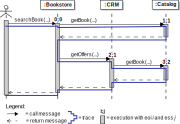
\includegraphics[width=0.96\columnwidth]{figures/eoiessBookstoreDemo-extended-2-combined}
\caption{UML Sequence Diagram illustrating our trace-related terminology}
\label{fig:exampleTraceTerminology}
\end{figure}

\begin{figure}\centering
% \vspace{-0.5cm}
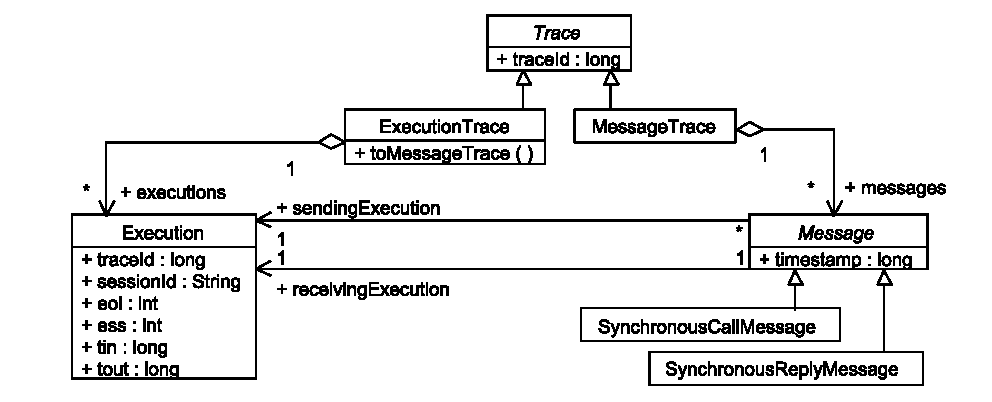
\includegraphics[scale=0.65]{figures/model/kieker_tracemodel}
% TR: 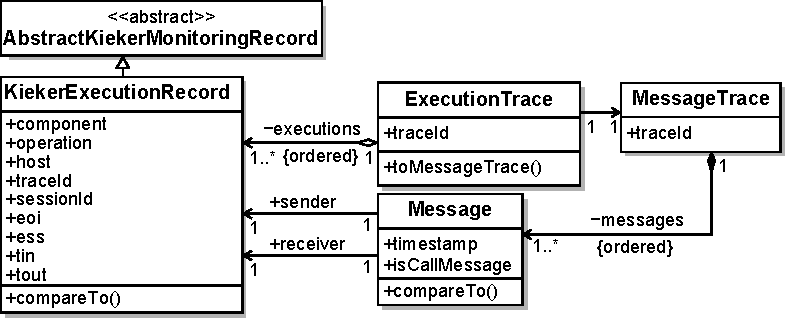
\includegraphics[width=1\columnwidth]{figures/kiekerTraceRepresentations-refined-bw}%
\caption{Trace meta-model used in Kieker.Tpan}
\label{fig:kiekerTraceRepresentations}
\end{figure}

\subsubsection{Logging Trace Information with \KiekerTpmon{}}

Kieker includes the \MonitoringRecord{} type \KiekerExecutionRecord{} which can %
be used to write \execution{} information into the \MonitoringLog{}. %
As shown in Figure~\ref{fig:kiekerTraceRepresentations}, an \KiekerExecutionRecord{} %
contains information about the executed \operation{}, the corresponding \component{}, 
the hostname on which the \execution{} was performed, as well as timestamps, %
typically with nanosecond resolution, for the start~(\textit{tin}) and end~(\textit{tout}) %
of an \execution{}. %
Kieker includes different \MonitoringProbe{} types for logging \KiekerExecutionRecords{} %
within an application, which look similar to the \MonitoringProbe{} in Listing~%
\ref{lst:aspectJRTMonitoringProbe}. %

A request to a system-provided service results in a nested control flow of %
corresponding \executions{}, referred to as a \textit{\trace{}}. %
Kieker provides efficient facilities for attaching a unique \traceIdentifier{} %
to the thread executing a service request, which is then contained in any %
\KiekerExecutionRecord{} of that \trace{}~(see~Figure~\ref{fig:kiekerTraceRepresentations}). 

\begin{lstlisting}[language=Java, float=*, numbers=none, xleftmargin=0pt,caption=Kieker.Tpan output of execution trace representation, label=lst:ExecutionRecordMonitoringLogExecutionTrace, basicstyle=\ttfamily\scriptsize]
TraceId 8430034814995791873 (NOSESSION):
<[0,0] 1257440666759412388-1257440666841265860 srv0::Bookstore.searchBook(..)>
<[1,1] 1257440666805601818-1257440666807695902 srv0::Catalog.getBook(..)>
<[2,1] 1257440666820790063-1257440666841169272 srv0::CRM.getOffers(..)>
<[3,2] 1257440666820839575-1257440666840922990 srv0::Catalog.getBook(..)>
\end{lstlisting}

%bin/tpan.sh -i /home/voorn/svn_work/pub_2009Kieker/tex-sources/tpmon-data/3_traceExample-tpmon-20091105-180426738/ -o tmp/ -p TSE --print-Execution-Trace
% \begin{lstlisting}[language=Java, float=*, numbers=none, xleftmargin=0pt, caption=Execution trace representation of trace~77, label=lst:ExecutionRecordMonitoringLogExecutionTrace, basicstyle=\ttfamily\small]
% <0 Bookstore.searchBook() .. 77 ..6759412388 ..6841265860 srv0 0 0 >
% <0 Catalog.getBook(boolean) .. 77 ..6805601818 ..6807695902 srv0 1 1 >
% <0 CRM.getOffers() .. 77 ..6820790063 ..6841169272 srv0 2 1 >
% <0 Catalog.getBook(boolean) .. 77 ..6820839575 ..6840922990 srv0 3 2 >
% \end{lstlisting}

%bin/tpan.sh -i /home/voorn/svn_work/pub_2009Kieker/tex-sources/tpmon-data/3_traceExample-tpmon-20091105-180426738/ -o tmp/ -p TSE --print-Message-Trace
% \begin{lstlisting}[language=Java, float=*, numbers=none, xleftmargin=0pt, caption=Message trace representation of trace~77, label=lst:ExecutionRecordMonitoringLogMessageTrace, basicstyle=\ttfamily\footnotesize]
% <..6759412388:$\$$|-send->Bookstore.searchBook()>
% <..6805601818:Bookstore|-send->Catalog.getBook(..)>
% <..6807695902:Catalog.getBook(..)|-return->Bookstore>
% <..6820790063:Bookstore|-send->CRM.getOffers()>
% <..6820839575:CRM|-send->Catalog.getBook(..)>
% <..6840922990:Catalog.getBook(..)|-return->CRM>
% <..6841169272:CRM.getOffers()|-return->Bookstore>
% <..6841265860:Bookstore.searchBook()|-return->$\$$>
% \end{lstlisting}
\begin{lstlisting}[language=Java, float=*, numbers=none, xleftmargin=0pt, caption=Kieker.Tpan output of message trace representation, label=lst:ExecutionRecordMonitoringLogMessageTrace, basicstyle=\ttfamily\scriptsize]
TraceId 8430034814995791873 (NOSESSION):
<SND 1257440666759412388 $\$$-->srv0::Bookstore.searchBook(..)[0,0]>
<SND 1257440666805601818 srv0::Bookstore.searchBook(..)[0,0]-->srv0::Catalog.getBook(..)[1,1]>
<RVC 1257440666807695902 srv0::Catalog.getBook(..)[1,1]-->srv0::Bookstore.searchBook(..)[0,0]>
<SND 1257440666820790063 srv0::Bookstore.searchBook(..)[0,0]-->srv0::CRM.getOffers(..)[2,1]>
<SND 1257440666820839575 srv0::CRM.getOffers(..)[2,1]-->srv0::Catalog.getBook(..)[3,2]>
<RVC 1257440666840922990 srv0::Catalog.getBook(..)[3,2]-->srv0::CRM.getOffers(..)[2,1]>
<RVC 1257440666841169272 srv0::CRM.getOffers(..)[2,1]-->srv0::Bookstore.searchBook(..)[0,0]>
<RVC 1257440666841265860 srv0::Bookstore.searchBook(..)[0,0]-->$\$$>
\end{lstlisting}

If the reconstruction of \traces{} from a \MonitoringLog{} containing \KiekerExecutionRecords{} %
would only include the \trace{} information presented so far, we would require the %
following assumptions: %
(a)~no two \execution{} start or end time events %
(\textit{tin}/\textit{tout}) within the same \trace{} occur at the same time; %
and (b)~clocks in a distributed system are perfectly synchronized (both with %
respect to the respective time resolution). %
Since both assumptions cannot be guaranteed in realistic environments, %
Kieker includes efficient facilities to attach two additional parameters to any %
\KiekerExecutionRecord{} in order to log the information needed to %
reconstruct (distributed)~\traces{} from the \MonitoringLog{} reliably: %
an \textit{\eoiLong{}~eoi} and an \textit{\essLong{}~ess}~(see~Figure~\ref{fig:kiekerTraceRepresentations}). %
\begin{description}
\item[eoi:] An \execution{} with an \eoiLong{} value~$i$ denotes the $i$-th %
\execution{} started within a \trace{} (starting with the value $0$).
\item[ess:] An \execution{} with an \essLong{} value~$j$ denotes an \execution{} that %
was started when the depth of the calling stack for the corresponding \trace{} was~$j$.
\end{description}

\noindent The \executions{} shown in the example \trace{} in Figure~\ref{fig:exampleTraceTerminology} 
are annotated with the corresponding \eoiLong{}~(eoi) and \essLong{}~(ess) values. %
Note, that while an \eoiLong{} is unique within a \trace{}, an \essLong{} %
value can, and usually does, occur more than once. %
% Listing~\ref{lst:ExecutionRecordMonitoringLog} shows the filesystem representation %
% of the \MonitoringLog{} for the example \trace{} of Figure~\ref{fig:exampleTraceTerminology}. %

\subsubsection{Trace Reconstruction with \KiekerTpan{}}

\begin{figure}\centering
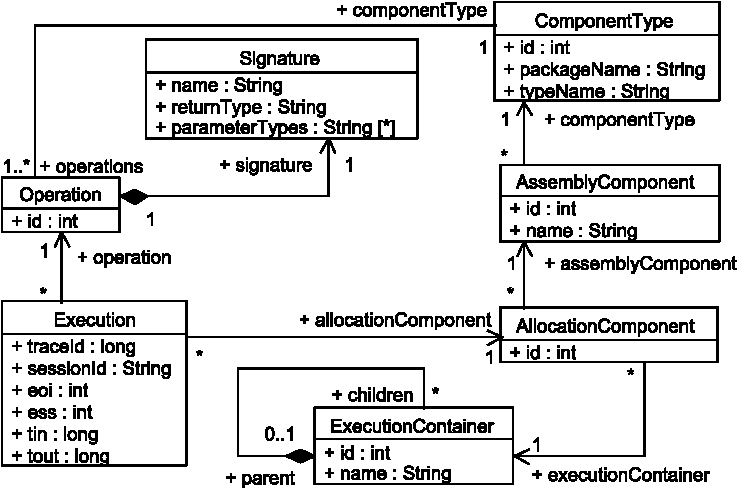
\includegraphics[scale=0.65]{figures/model/kieker_systemmodel-crop}
\caption{System meta-model used in Kieker.Tpan}
\end{figure}


In \KiekerTpan{}, two equivalent representations of \traces{} are used internally: %
\executionTraces{} and \messageTraces{}. %
An \executionTrace{} representation of a \trace{} is simply the ordered~(by %
\eoiLong{} values) sequence of \executions{}~(stored as \KiekerExecutionRecords{}, see Figure~\ref{fig:kiekerTraceRepresentations}). %
A~\messageTrace{} describes a \trace{} in terms of an ordered sequence of \Messages{} %
instead of \executions{}. %
Each \execution{} can be described by a corresponding \callMessage{}, %
representing an \operation{} call which starts the \execution{}, %
and a \returnMessage{}, representing the end of an \execution{} returning the %
control flow to the calling \execution{}, as illustrated in Figure~\ref{fig:exampleTraceTerminology}. %
For more details, refer to the associations \sender{} and \receiver{} in Figure~\ref{fig:kiekerTraceRepresentations}.
Listings~\ref{lst:ExecutionRecordMonitoringLogExecutionTrace} and \ref{lst:ExecutionRecordMonitoringLogMessageTrace} %
show text representations of the corresponding \executionTrace{} and a \messageTrace{} stored by \KiekerTpan{}, respectively.

Figure~\ref{fig:kiekerTraceRepresentations} shows the relations among \executions{}, %
\Messages{}, \executionTraces{}, and \messageTraces{}. %
While it is straightforward to derive \executionTraces{} from the \MonitoringLog{}, %
for later analysis it is usually easier to derive analysis models from \messageTraces{}. %
In \KiekerTpan{}, \executionTraces{} are derived from the \MonitoringLog{} and %
then transformed into equivalent \messageTrace{} representations from which %
analysis models and diagrams, as described in the following \mbox{Section~%
\ref{sec:traceAnalysisAndVisualization}}, are created.

% Underlying assumption: Each request is serviced by a trace of (nested) synchronous executions.

% In order to emphasize the caller/callee relationship among \components{} involved %
% in an \execution{} of an \operation{}, a message-oriented view can be taken by
% associating two types of \Messages{} with an \execution{}: %
% a \textit{\callMessage{}} and a \textit{\returnMessage{}}. %

% Implemented for distributed Web service scenarios (SOAP/cxf)

% \paragraph{From Execution Traces to Message Traces}\
% 
% Execution trace representation:
% \begin{itemize}
% \item Ordered set of executions (ordered by eoi)
% \item The monitoring log contains the unsorted executions
% \end{itemize}
% 
% Message trace representation:
% \begin{itemize}
% \item Ordered set of call/return messages
% \item Can easily be constructed from execution trace%\footnote{See {\scriptsize\texttt{kieker.loganalysis.datamodel.ExecutionTrace.toMessageTrace()}}\\}
% \item[$\rightarrow$] Straight-forward transformation to\\ sequence diagrams, dependency graphs, ...
% \end{itemize}
% 
% \TODOBOX{Show Algorithm}
% 
\subsection{Analysis and Visualization of Trace Information}\label{sec:traceAnalysisAndVisualization}

\begin{figure}\centering
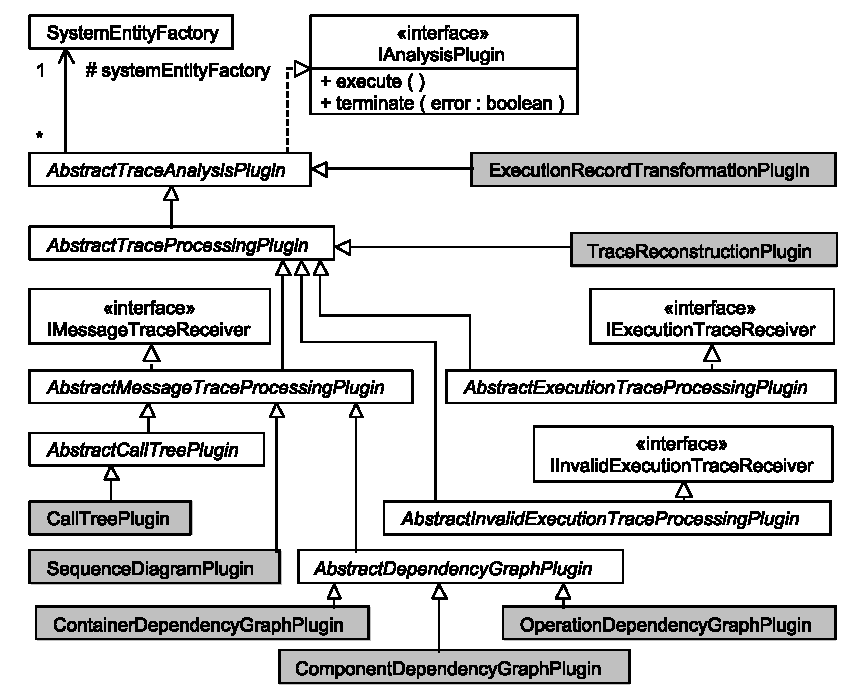
\includegraphics[scale=0.65]{figures/model/kieker_traceprocessingcomponents}
\caption{Trace analysis plugins in Kieker.Tpan}
\label{fig:traceAnalysisPlugins}
\end{figure}

\begin{figure}\centering
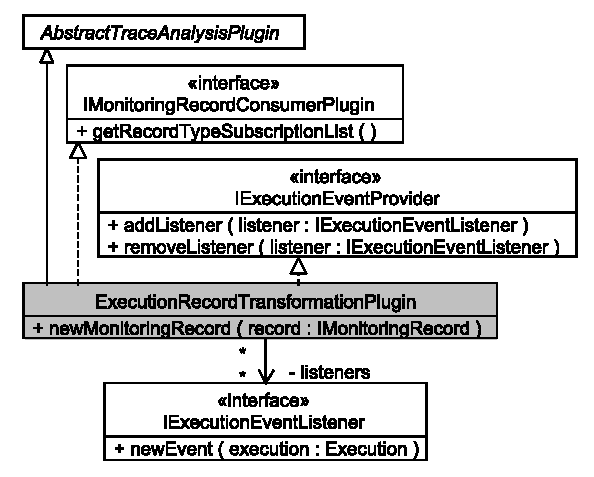
\includegraphics[scale=0.65]{figures/model/kieker_executionRecordTransformer}
\caption{Execution record transformation plugin}
\label{fig:execRecordTransformationPlugin}
\end{figure}

\begin{figure}\centering
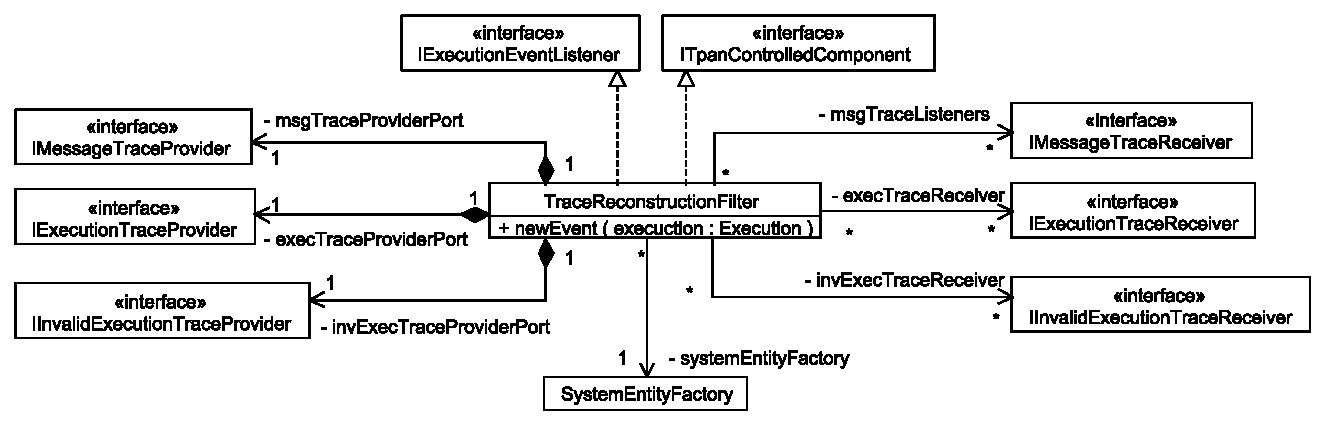
\includegraphics[scale=0.65]{figures/model/kieker_traceReconstructionFilter}
\caption{Trace reconstruction plugin}
\label{fig:traceReconstructionPlugin}
\end{figure}

\noindent As described in the previous Section~\ref{sec:traceLoggingAndReconstruction}, %
\KiekerTpmon{} allows to log (distributed)~trace information to the \MonitoringLog{} %
which can then be transformed into two equivalent \trace{} representations using %
\KiekerTpan{}, i.e., \executionTraces{} and \messageTraces{}. %
These representations constitute the basis for \trace{}-based analysis and 
visualization functionality which can be integrated into the \KiekerTpan{} %
component. %
This section gives an overview of some of the \trace{}-based analysis and visualization %
functionality which have been integrated into \KiekerTpan{} so far: sequence diagrams, dynamic call trees, dependency diagrams, and Markov chains. %
By implementing a \MonitoringRecordConsumer{}, as described in Section~\ref{sec:architecture}, %
it is easy to implement custom components for analyzing and visualizing \trace{} %
information employing the Kieker framework.

%
% JPetStore dataset 3_20090710-163529-jpetstore-250Threads-400sDuration-200sRampup/
% 
% 236719 traces

\begin{figure}\centering
% TR:
% bin/tpan.sh -i 3_20090710-163529-jpetstore-250Threads-400sDuration-200sRampup/tpmon-20090710-163529/ -p JPET --plot-Sequence-Diagram -o tmp/
% pic2plot -T svg tmp/JPETsequenceDiagram-19503.pic > tmp/JPETsequenceDiagram-19503.svg
% # removed package names in method signature w/ inkscape -> export to eps
% epstopdf sequenceDiagram-19503-noPackageName.eps
% \vspace{-0.3cm}
% 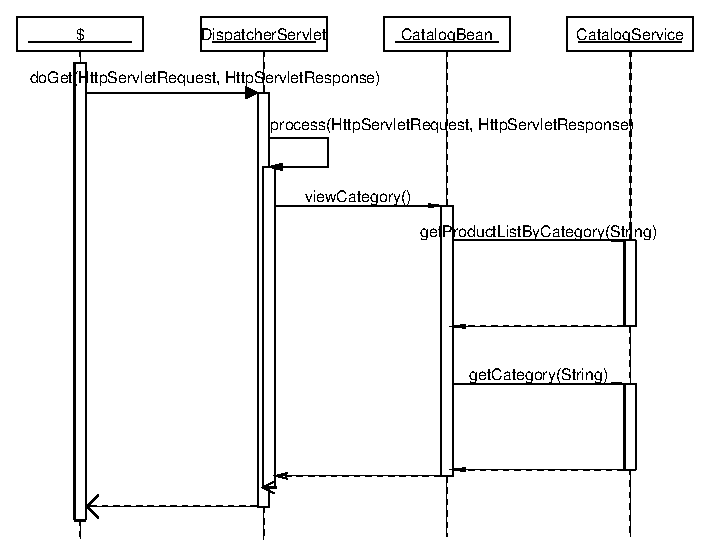
\includegraphics[width=\columnwidth]{figures/20090710-163529-jpetstore-250Threads-400sDuration-200sRampup-sequenceDiagram-19503}%

% bin/trace-analysis.sh -i /home/voorn/svn_work/sw_kieker/trunk/documentation/architecture/tex-sources/tpmon-testdata/3_20090710-163529-jpetstore-250Threads-400sDuration-200sRampup/tpmon-20090710-163529-filtered/ -p JPET --plot-Sequence-Diagrams -o tmp/ --select-traces 19503 --short-labels
%pic2plot -T ps /home/voorn/svn_work/sw_kieker/branches/1.1-refactoring/tmp/JPETsequenceDiagram-19503.pic > /home/voorn/svn_work/sw_kieker/branches/1.1-refactoring/tmp/JPETsequenceDiagram-19503.ps
%ps2pdf ... && pdfcrop
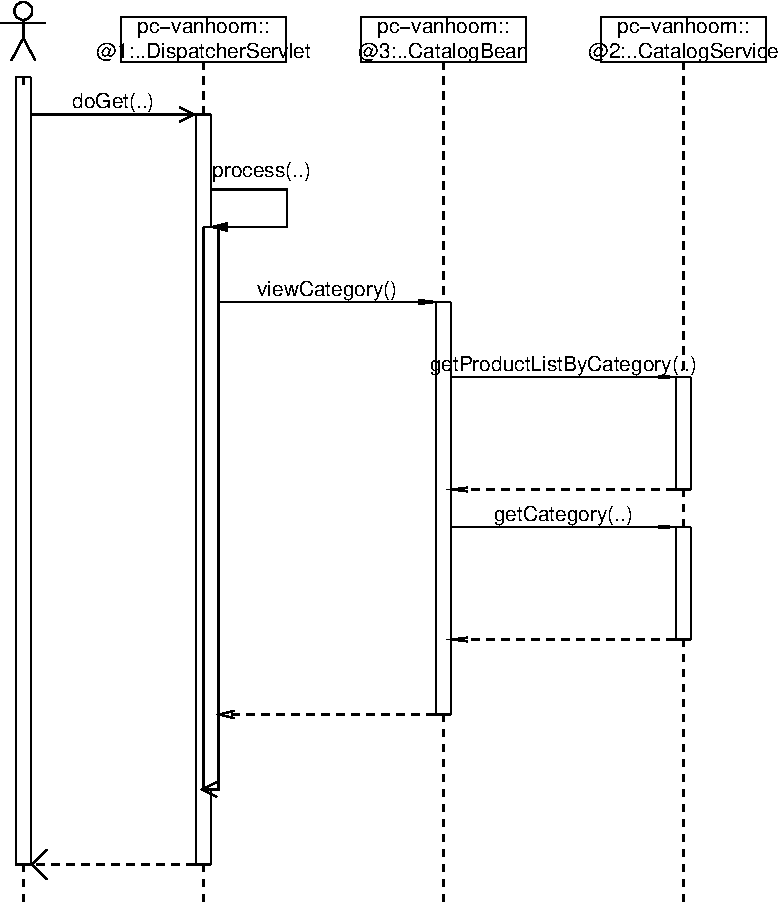
\includegraphics[width=0.8\columnwidth]{figures/20090710-163529-jpetstore-250Threads-400sDuration-200sRampup-sequenceDiagram-19503--20100428-crop}%

\caption{UML sequence diagram generated by Kieker.Tpan}
\label{fig:vis:jpetSeqDiagr}
\end{figure}

\subsubsection{UML~sequence diagrams}

UML~sequence diagrams provide a dynamic architectural viewpoint in terms %
of interactions among runtime objects implementing software services. %
In Figure~\ref{fig:exampleTraceTerminology} of the previous section, we used %
a sequence diagram to illustrate the \trace{}-related terminology needed to define %
\executionTraces{} and \messageTraces{}. %
\MessageTraces{} can be transformed to UML~sequence diagrams in a straightforward way. %
Figure~\ref{fig:vis:jpetSeqDiagr} shows such a UML sequence diagram generated by %
a Kieker visualization component for the iBATIS JPetStore which is a demo Java Web application implementing an
online store scenario.\footnote{The case study iBATIS JPetStore from \url{http://ibatis.apache.org/} is available as an instrumented version on the Kieker web page \url{http://kieker.sourceforge.net/}.} We employ this case study to give examples for visualizations in the present section. %
Given the timing information included in the \executionTraces{}, the sequence diagrams %
could easily be augmented with this additional data, e.g., observed response %
times. The UML~specification~\citep{OMG2007UML22Superstructure} and %
the UML~profiles for performance~\citep{OMG2005UMLProfileForSchedulabilityPerformanceAndTimeV1-1,OMG2008UMLProfileForMARTEBeta2} %
suggest appropriate notations for performance annotations. %
%Adding UML's combined fragments, e.g., loops and optional behavior, would only require %
%the definition of suitable \MonitoringRecords{} and corresponding \MonitoringProbes{} %
%collecting this information.\MR{Zum letzten Satz: Kann man loops etc. wirklich so einfach erkennen? Ich glaube da muss man mehr in der Analyse machen, wie soll das Monitoring einen Loop erkennen (Loop-Erkennung ist ein Problem fuer sich)... Besser den letzten Satz streichen, da wir es noch nicht bieten.}

\subsubsection{Dynamic call trees}

% bin/trace-analysis.sh -i /home/voorn/svn_work/sw_kieker/trunk/documentation/architecture/tex-sources/tpmon-testdata/3_20090710-163529-jpetstore-250Threads-400sDuration-200sRampup/tpmon-20090710-163529-filtered/ -p 20090710-163529-jpetstore-250Threads-400sDuration-200sRampup--20100428-  -o tmp/ --select-traces 61 --short-labels --plot-Call-Trees

% TR:
% \begin{figure}\centering
% 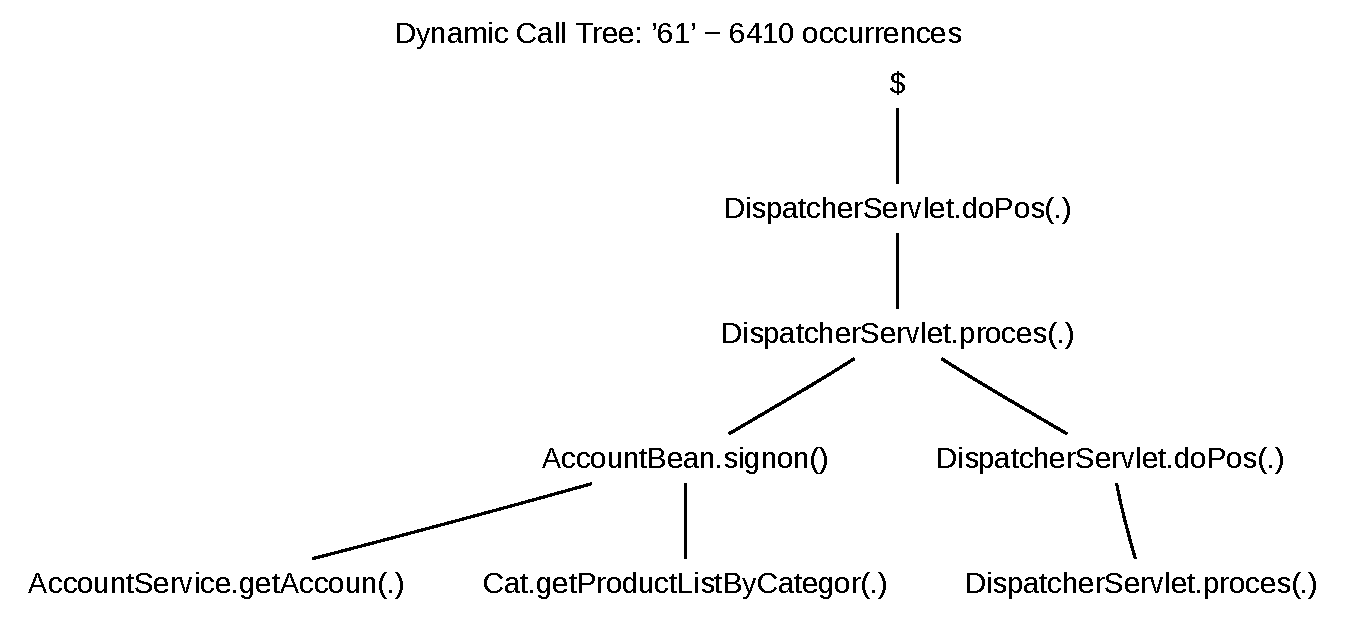
\includegraphics[width=\columnwidth]{figures/20090710-163529-jpetstore-250Threads-400sDuration-200sRampup-dynamicCallTree61}
% \caption{Call tree corresponding to a trace equivalence class generated by Kieker.Tpan}
% \label{fig:vis:jpetDepCallTree}
% \end{figure}

\begin{figure}\centering
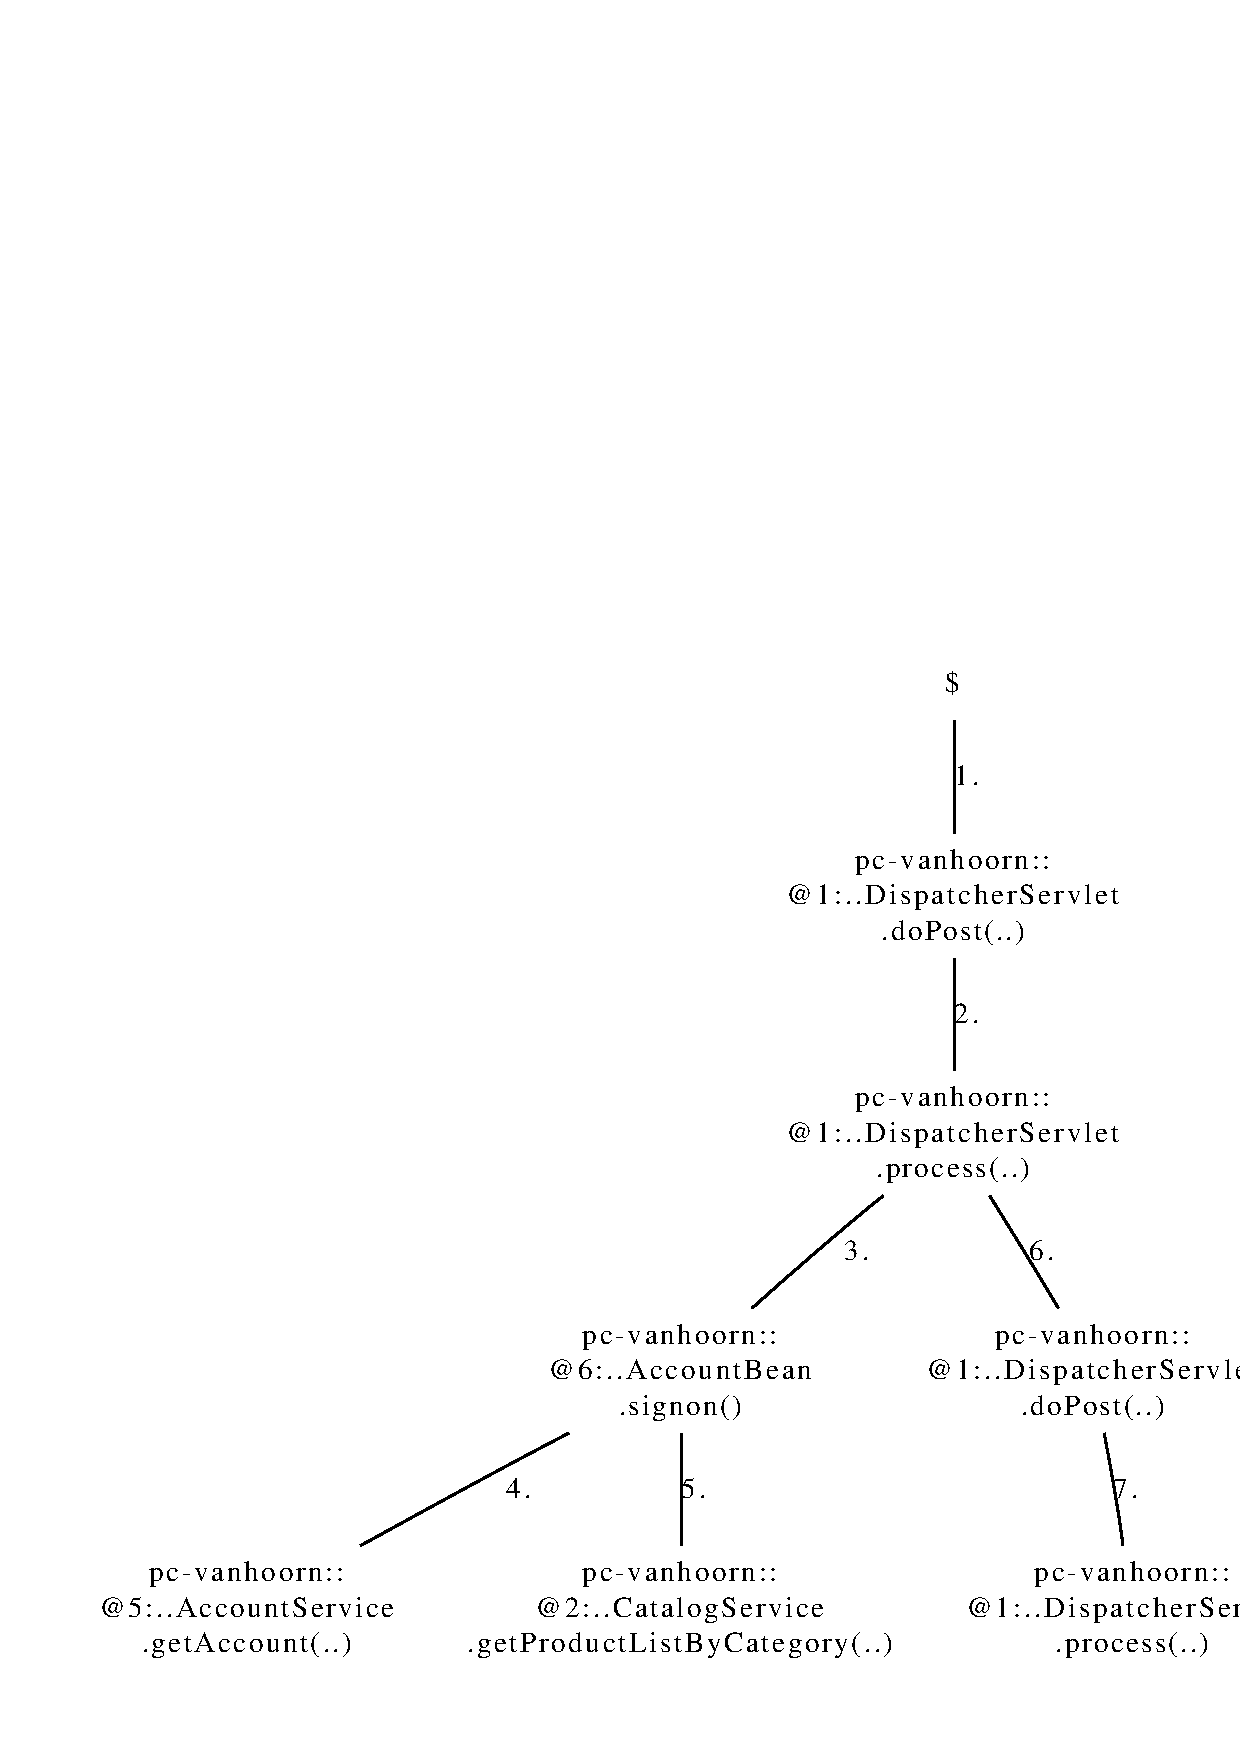
\includegraphics[width=\columnwidth]{figures/20090710-163529-jpetstore-250Threads-400sDuration-200sRampup-sequenceDiagram--20100428-callTree-61}
\caption{Call tree corresponding to a single trace% generated by Kieker.Tpan
}
\label{fig:vis:jpetDepCallTree}
\end{figure}

\begin{figure}\centering
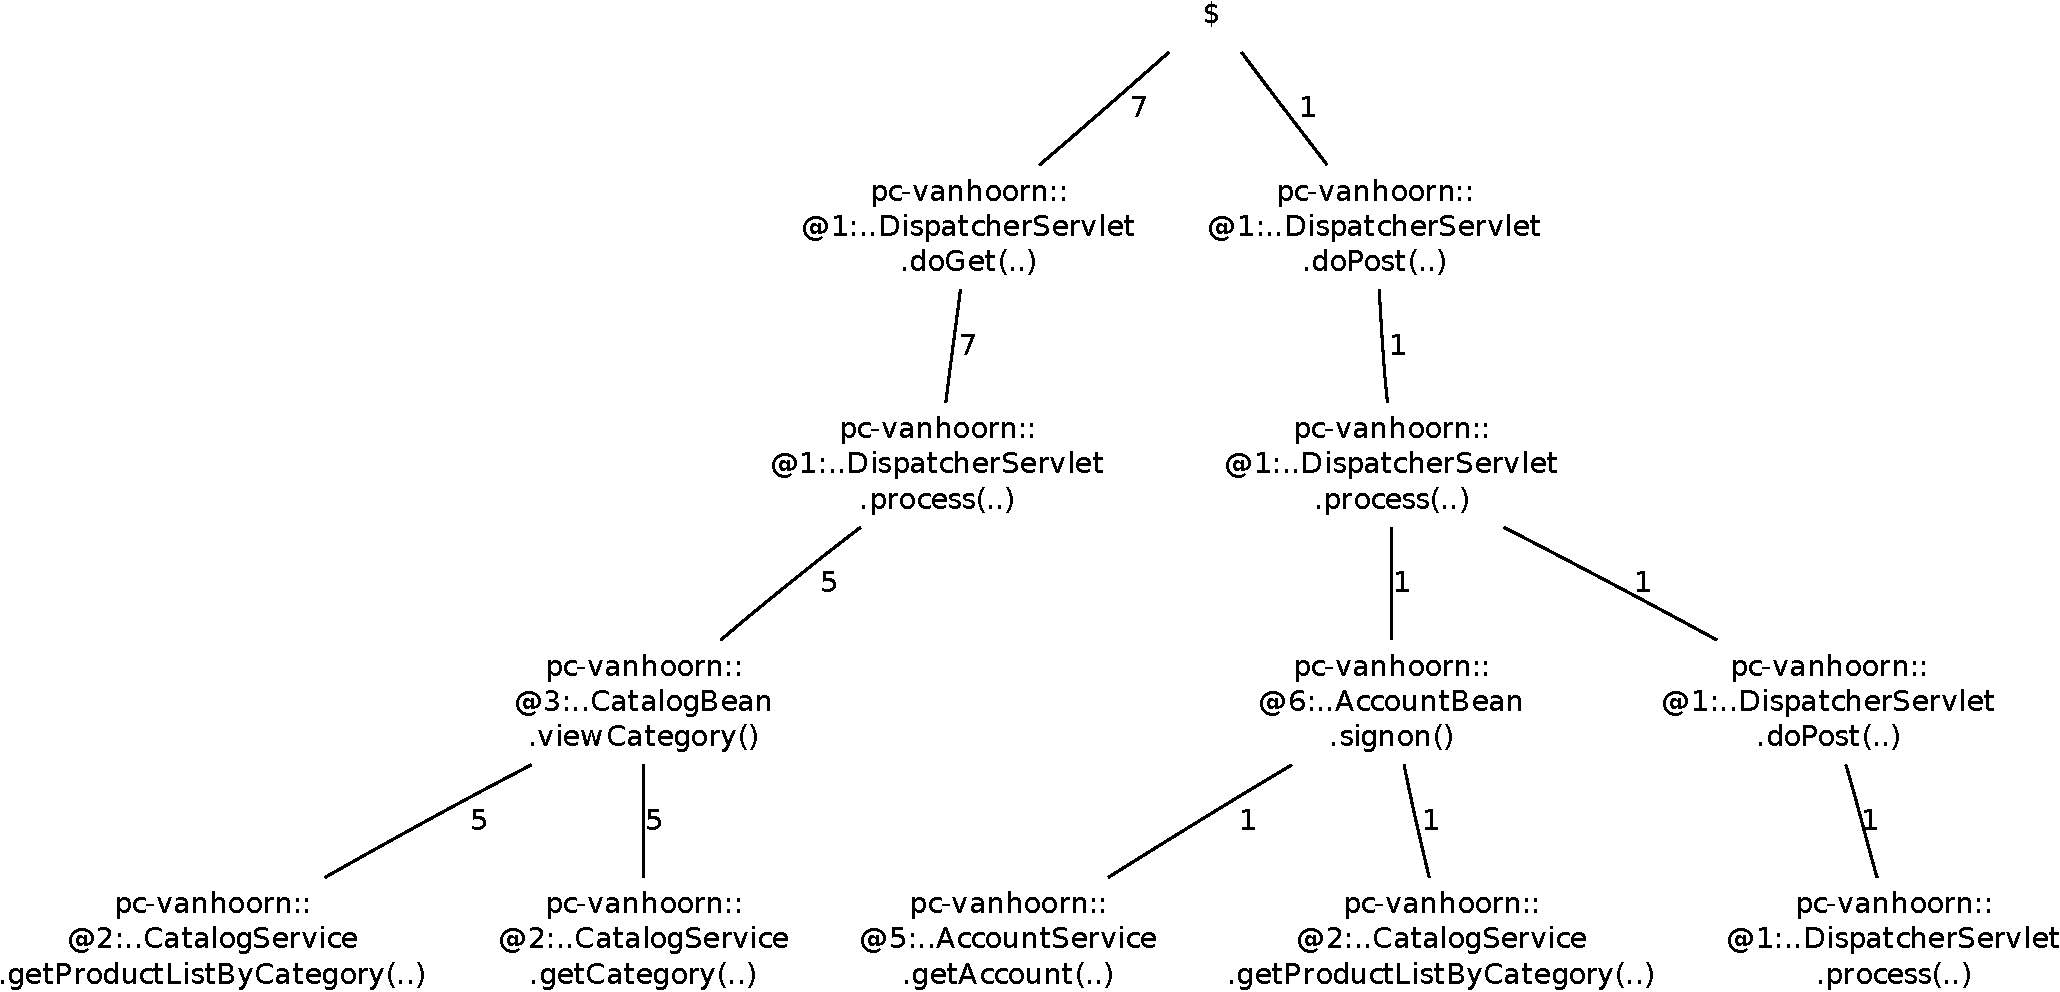
\includegraphics[width=\columnwidth]{figures/20090710-163529-jpetstore-250Threads-400sDuration-200sRampup--20100428-aggregatedCallTree}
\caption{Aggregated call tree corresponding to 8 traces% generated by Kieker.Tpan
}
\label{fig:vis:jpetDepAggregatedCallTree}
\end{figure}

Figure~\ref{fig:vis:jpetDepCallTree} shows an alternative representation of %
a \trace{}, called \textit{dynamic call tree}%
%\MR{Achtung! Habe `call tree' in `dynamic call tree' umbenannt (siehe Referenz AmmonsBallLarus97 S. 5)}
~\citep{AmmonsBallLarus97ExploitingHardwarePerformanceCountersWithFlowAndContextSensitiveProfiling}, generated by \KiekerTpan{}. A dynamic call tree %
contains the calling relations (\callMessages{}) among \operations{}, in contrast %
to a sequence diagram which also includes the corresponding \returnMessages{}. A dynamic call tree is an ordered graph, where the order (left to right) corresponds to the execution order of the nodes.
In~\citep{RohrvanHoornGieseckeMatevskaHasselbringAlekseev2008TraceContextSensitivePerformanceProfilingForEnterpriseSoftwareApplications}, %
we use the control flow information contained in a dynamic call tree to %
analyze the recorded response times of \operations{} based on the call tree position of the %
corresponding \executions{}.

When analyzing \traces{} from the \MonitoringLog{}, a valuable initial analysis %
is to determine the \trace{} \textit{equivalence classes}. %
Informally, a \trace{} equivalence class contains all \traces{} which are equal %
in terms of the control flow, i.e., the sequence diagrams of all \traces{} in an 
equivalence class are identical. %
Based on the \messageTraces{} this analysis can be implemented efficiently. %
Figure~\ref{fig:vis:jpetDepCallTree} shows the dynamic call tree common to all 6\,410~\traces{} %
in a \trace{} equivalence class extracted from the monitoring data of the JPetStore example. %

\subsubsection{Dependency graphs}

% TR:
% \begin{figure*}\centering
% % bin/tpan.sh -i 3_20090710-163529-jpetstore-250Threads-400sDuration-200sRampup/tpmon-20090710-163529/ -p JPET --plot-Dependency-Graph -o tmp/
% % dot -T eps tmp/JPETdependencyGraph.dot > tmp/JPETdependencyGraph.eps
% % epstopdf tmp/JPETdependencyGraph.eps
% 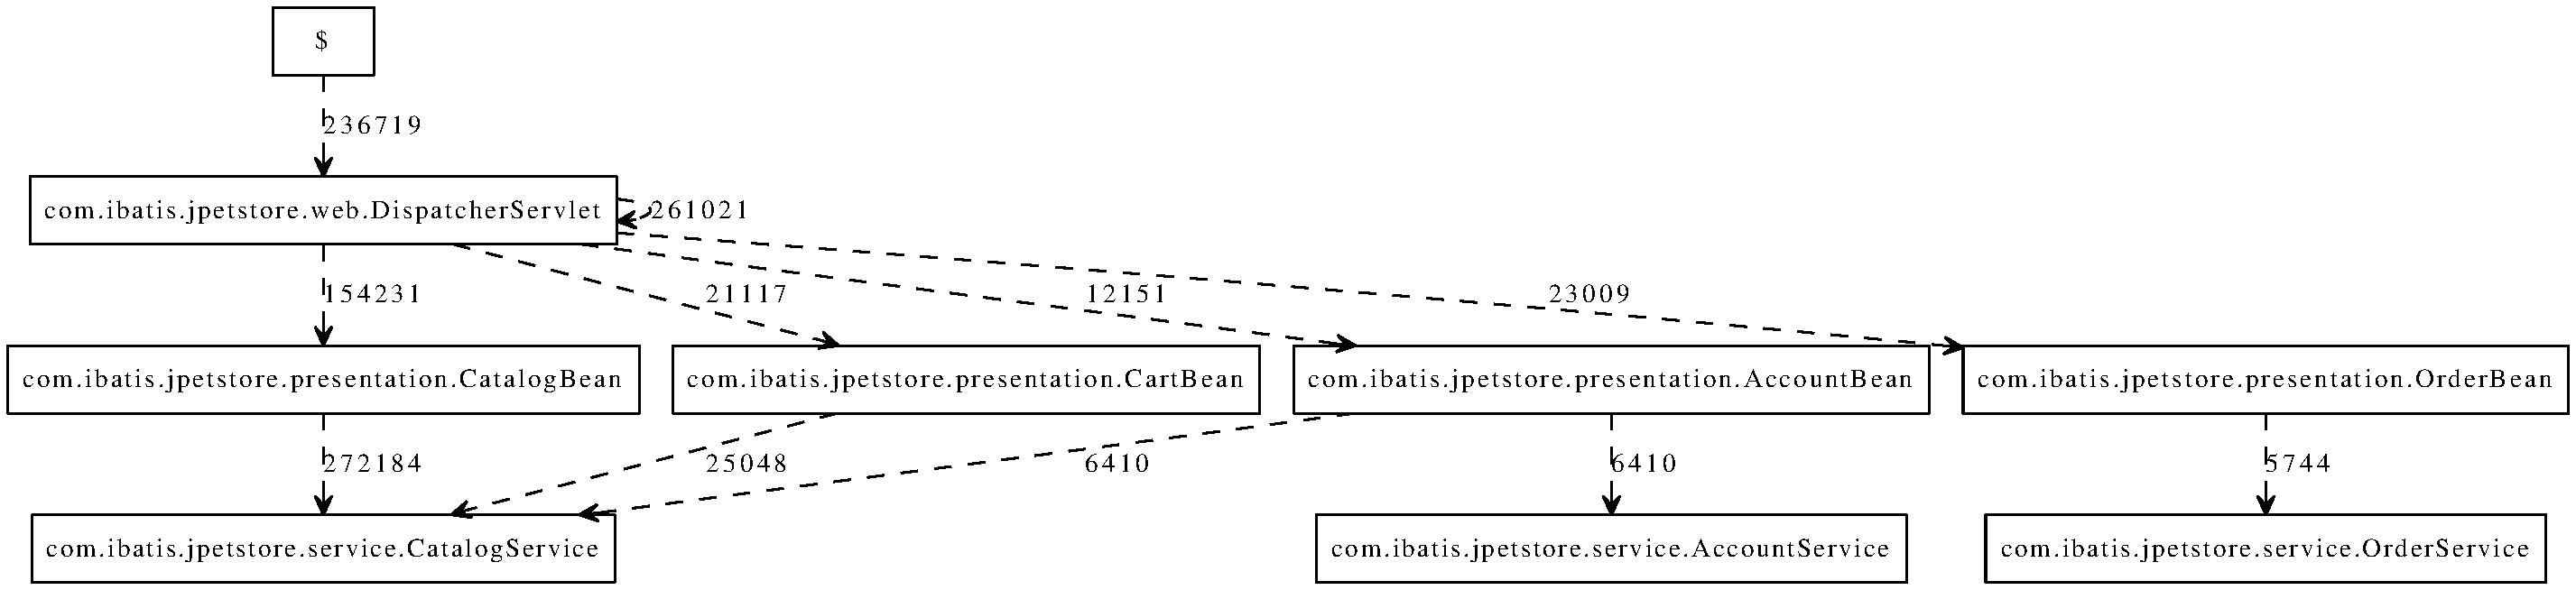
\includegraphics[width=\textwidth]{figures/20090710-163529-jpetstore-250Threads-400sDuration-200sRampup-dependencyGraph}%
% \caption{Component dependency graph visualization generated by Kieker.Tpan}
% \label{fig:vis:jpetDepDiagr}
% \end{figure*}

% bin/trace-analysis.sh -i /home/voorn/svn_work/sw_kieker/trunk/documentation/architecture/tex-sources/tpmon-testdata/3_20090710-163529-jpetstore-250Threads-400sDuration-200sRampup/tpmon-20090710-163529-filtered/ -p 20090710-163529-jpetstore-250Threads-400sDuration-200sRampup-sequenceDiagram--20100428- -o tmp/ --short-labels --plot-Component-Dependency-Graph --plot-Container-Dependency-Graph --plot-Operation-Dependency-Graph
\begin{figure}\centering
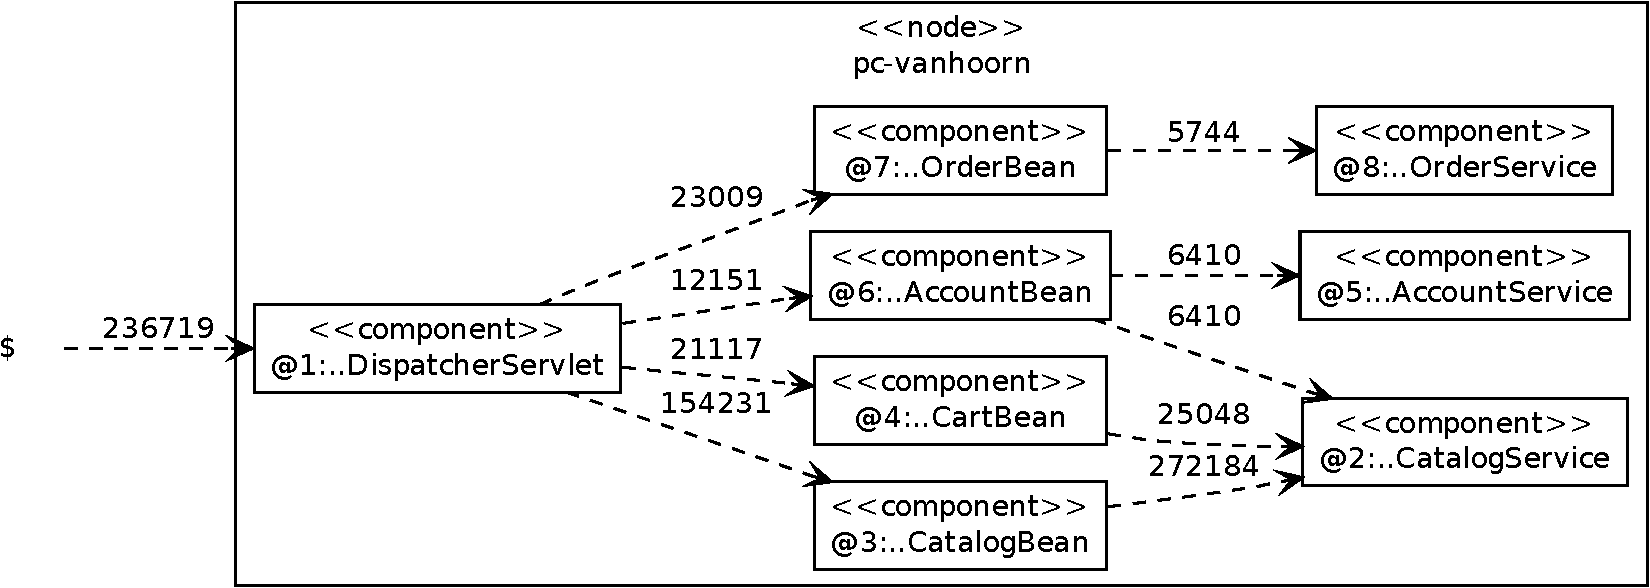
\includegraphics[width=\columnwidth]{figures/20090710-163529-jpetstore-250Threads-400sDuration-200sRampup-sequenceDiagram--20100428-componentDependencyGraph}%
\caption{Component dependency graph visualization %generated by Kieker.Tpan
}
\label{fig:vis:jpetComponentDepDiagr}
\end{figure}

\begin{figure}\centering
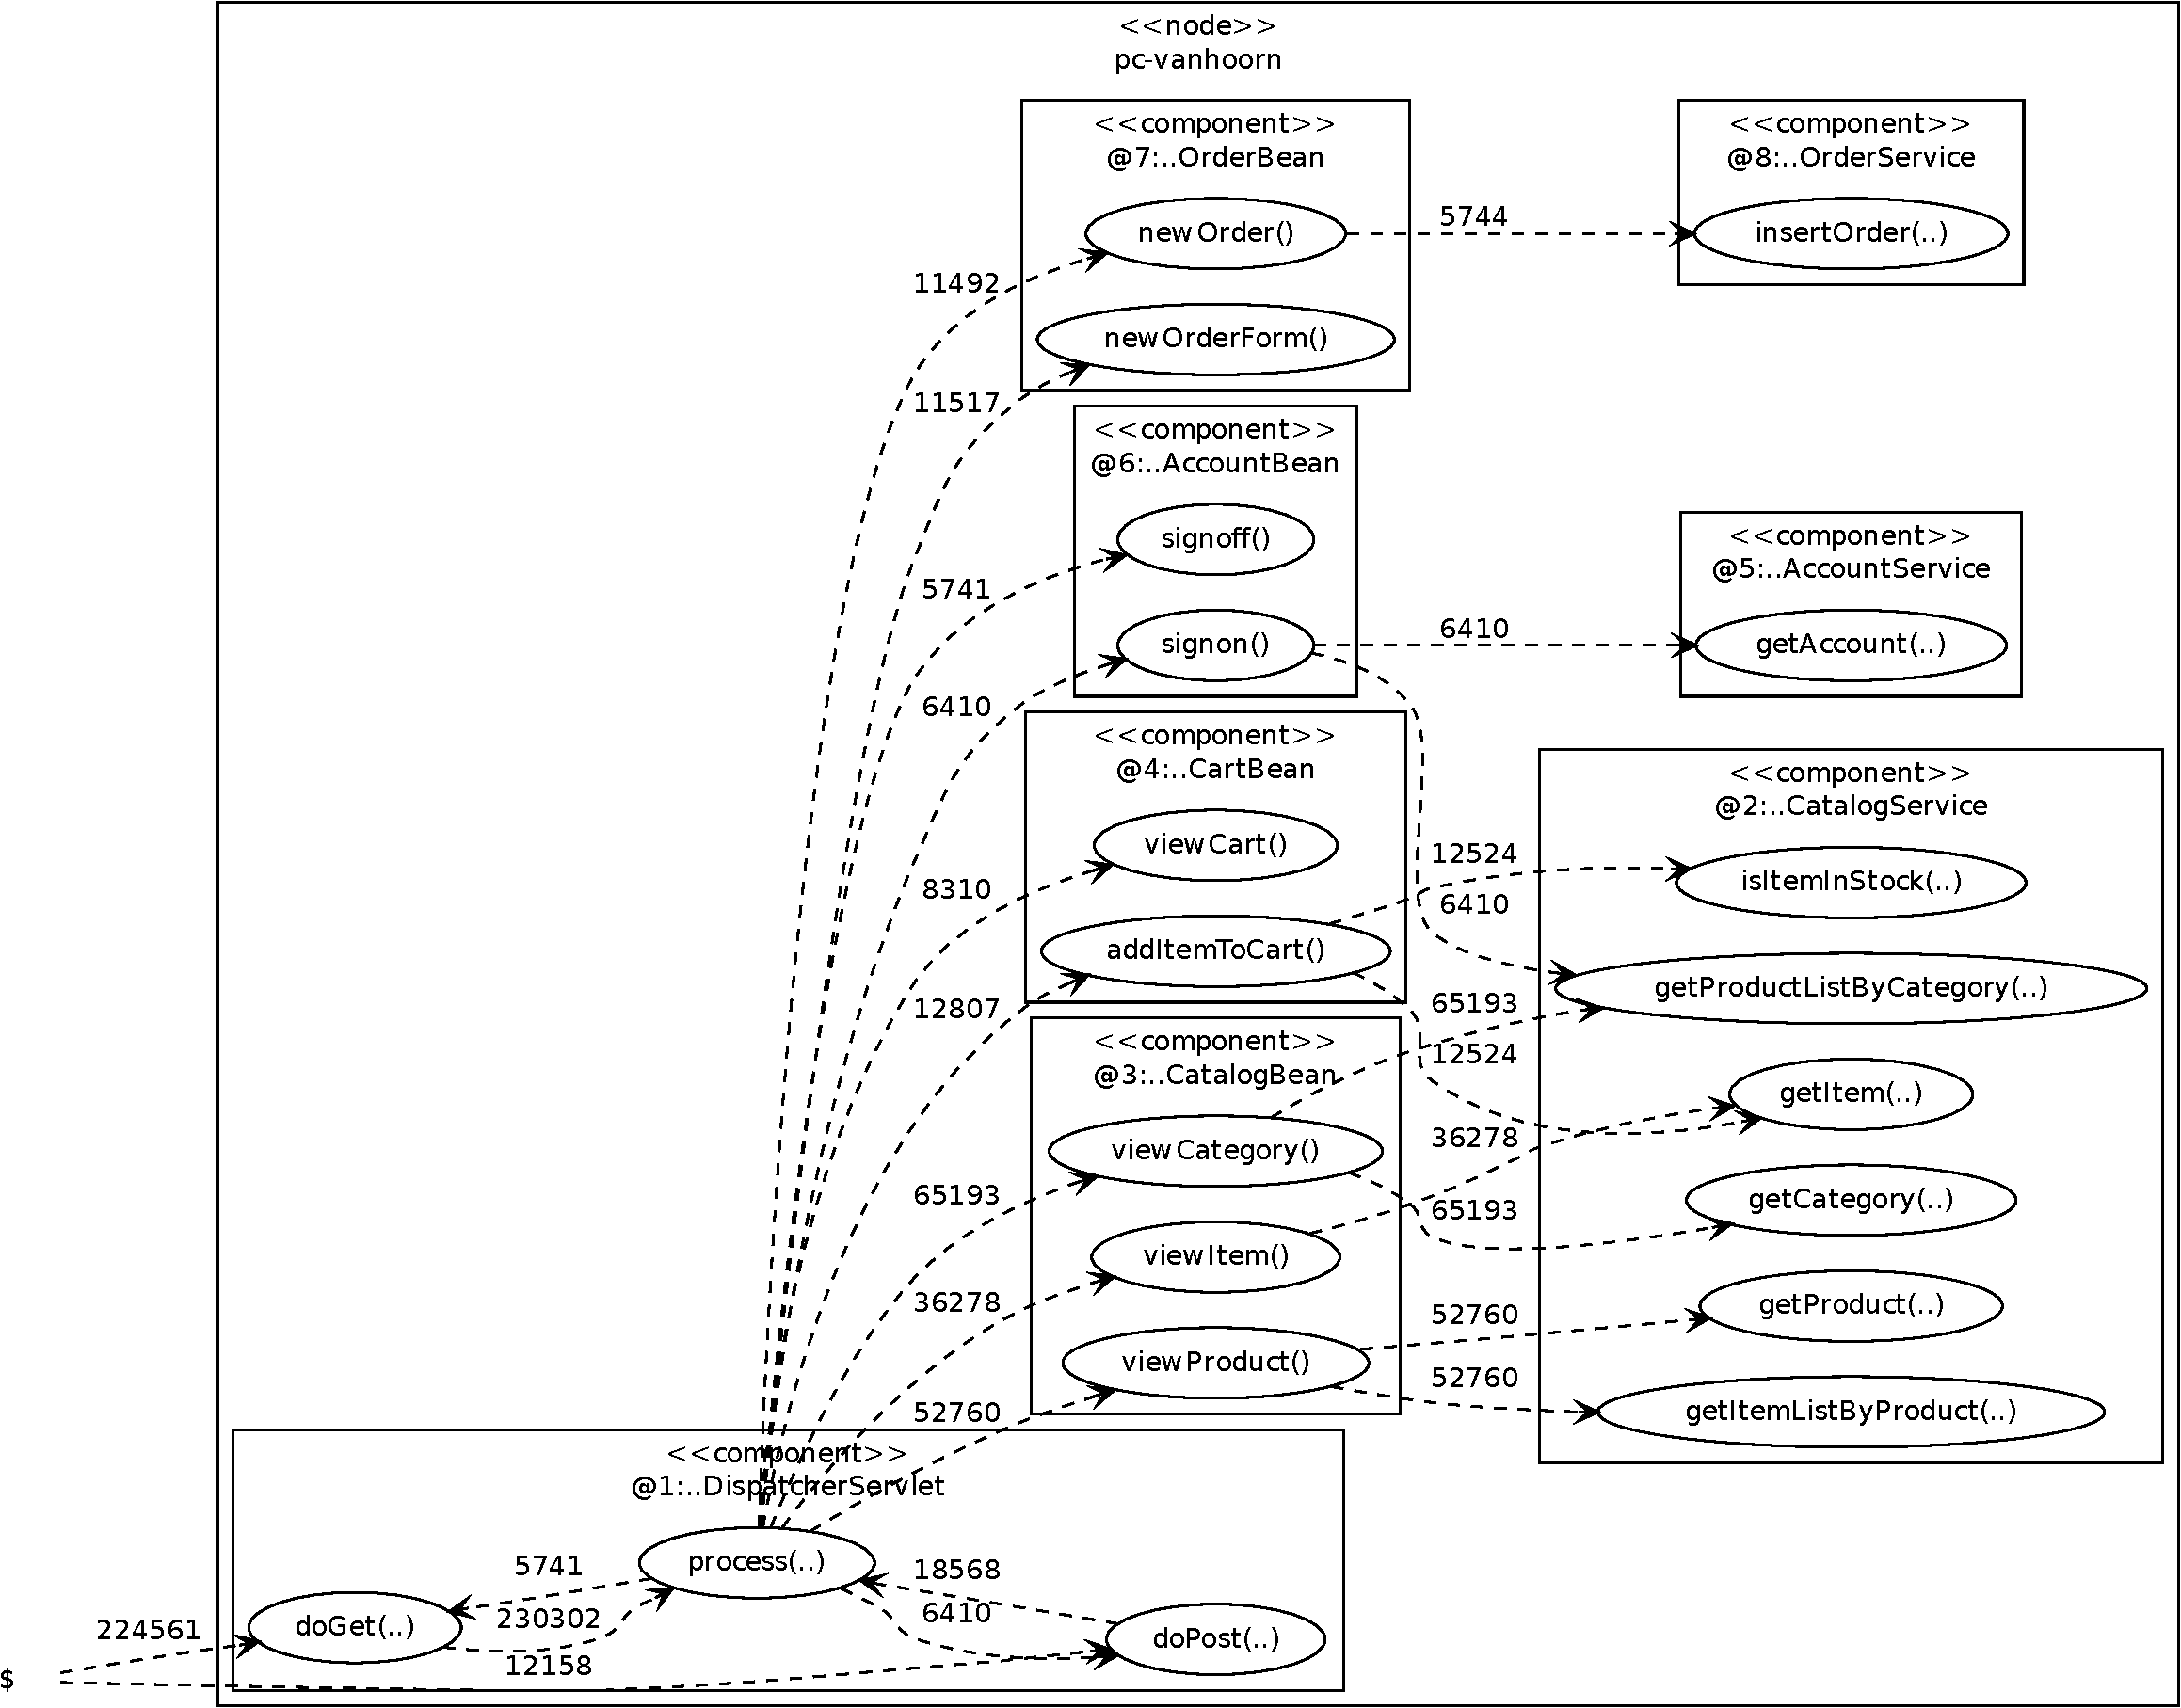
\includegraphics[width=\columnwidth]{figures/20090710-163529-jpetstore-250Threads-400sDuration-200sRampup-sequenceDiagram--20100428-operationDependencyGraph}%
\caption{Operation dependency graph visualization% generated by Kieker.Tpan
}
\label{fig:vis:jpetOperationDepDiagr}
\end{figure}

While sequence diagrams, or \executionTraces{}, provide a view on the \textit{sequence} of %
interactions among objects in a single \trace{} (or scenario/use~case), it is often %
desirable to analyze this information in an aggregated %\MR{Ist es ganz klar ueber was man aggregiert?} 
form. %
Interactions among objects constitute runtime dependencies among these system %
entities, which can be described using weighted directed dependency graphs: %
each entity is assigned a node and each dependency relation %
an edge; the edge is directed from an entity using %(calling)
a particular service to the entity providing that service; 
the edges are augmented with the total number of call actions %\MR{actions statt messages? (UML)} 
among the respective entities observed in the considered set of \traces{}. %

We implemented a \KiekerTpan{} component which computes dependency graphs, %
% calling dependencies from \executionTraces{}, %
represented in adjacency matrices, from a set of \messageTraces{}. %
These dependency graphs are then available for further analysis or visualization. %
Figure~\ref{fig:vis:jpetDepDiagr} shows a dependency graph generated by %
\KiekerTpan{}, visualizing calling dependencies among classes of the partly-instrumented %
JPetStore application. The figure provides an aggregated view of the runtime dependencies %
observed in 236\,719~traces, resulting from 250~concurrent users simulated by probabilistic %
workload generation~\citep{vanHoornRohrHasselbring2008GeneratingProbabilisticAndIntensityVaryingWorkloadForWebBasedSoftwareSystems}. %

% In addition to dependencies among components~(or classes in this example), %
% \executionTraces{} allow to compute dependencies among execution contexts~(hosts) %
% and operations, which can then be represented as hierarchical dependency graphs. %
% Figure~\ref{fig:hierarchicalDependecyGraph} shows a drill-down view of a hierarchical %
% dependency graph, with weighted dependencies among deployment contexts, components, 
% and operations. The graph is augmented with failure diagnosis results based on 
% timing behavior analysis detailed in~\citep{MarwedeRohrHoornHasselbring2009AutomaticFailureDiagnosisInDistributedLargeScaleSoftwareSystemsBasedOnTimingBehaviorAnomalyCorrelation}.

% \begin{figure}\centering
% 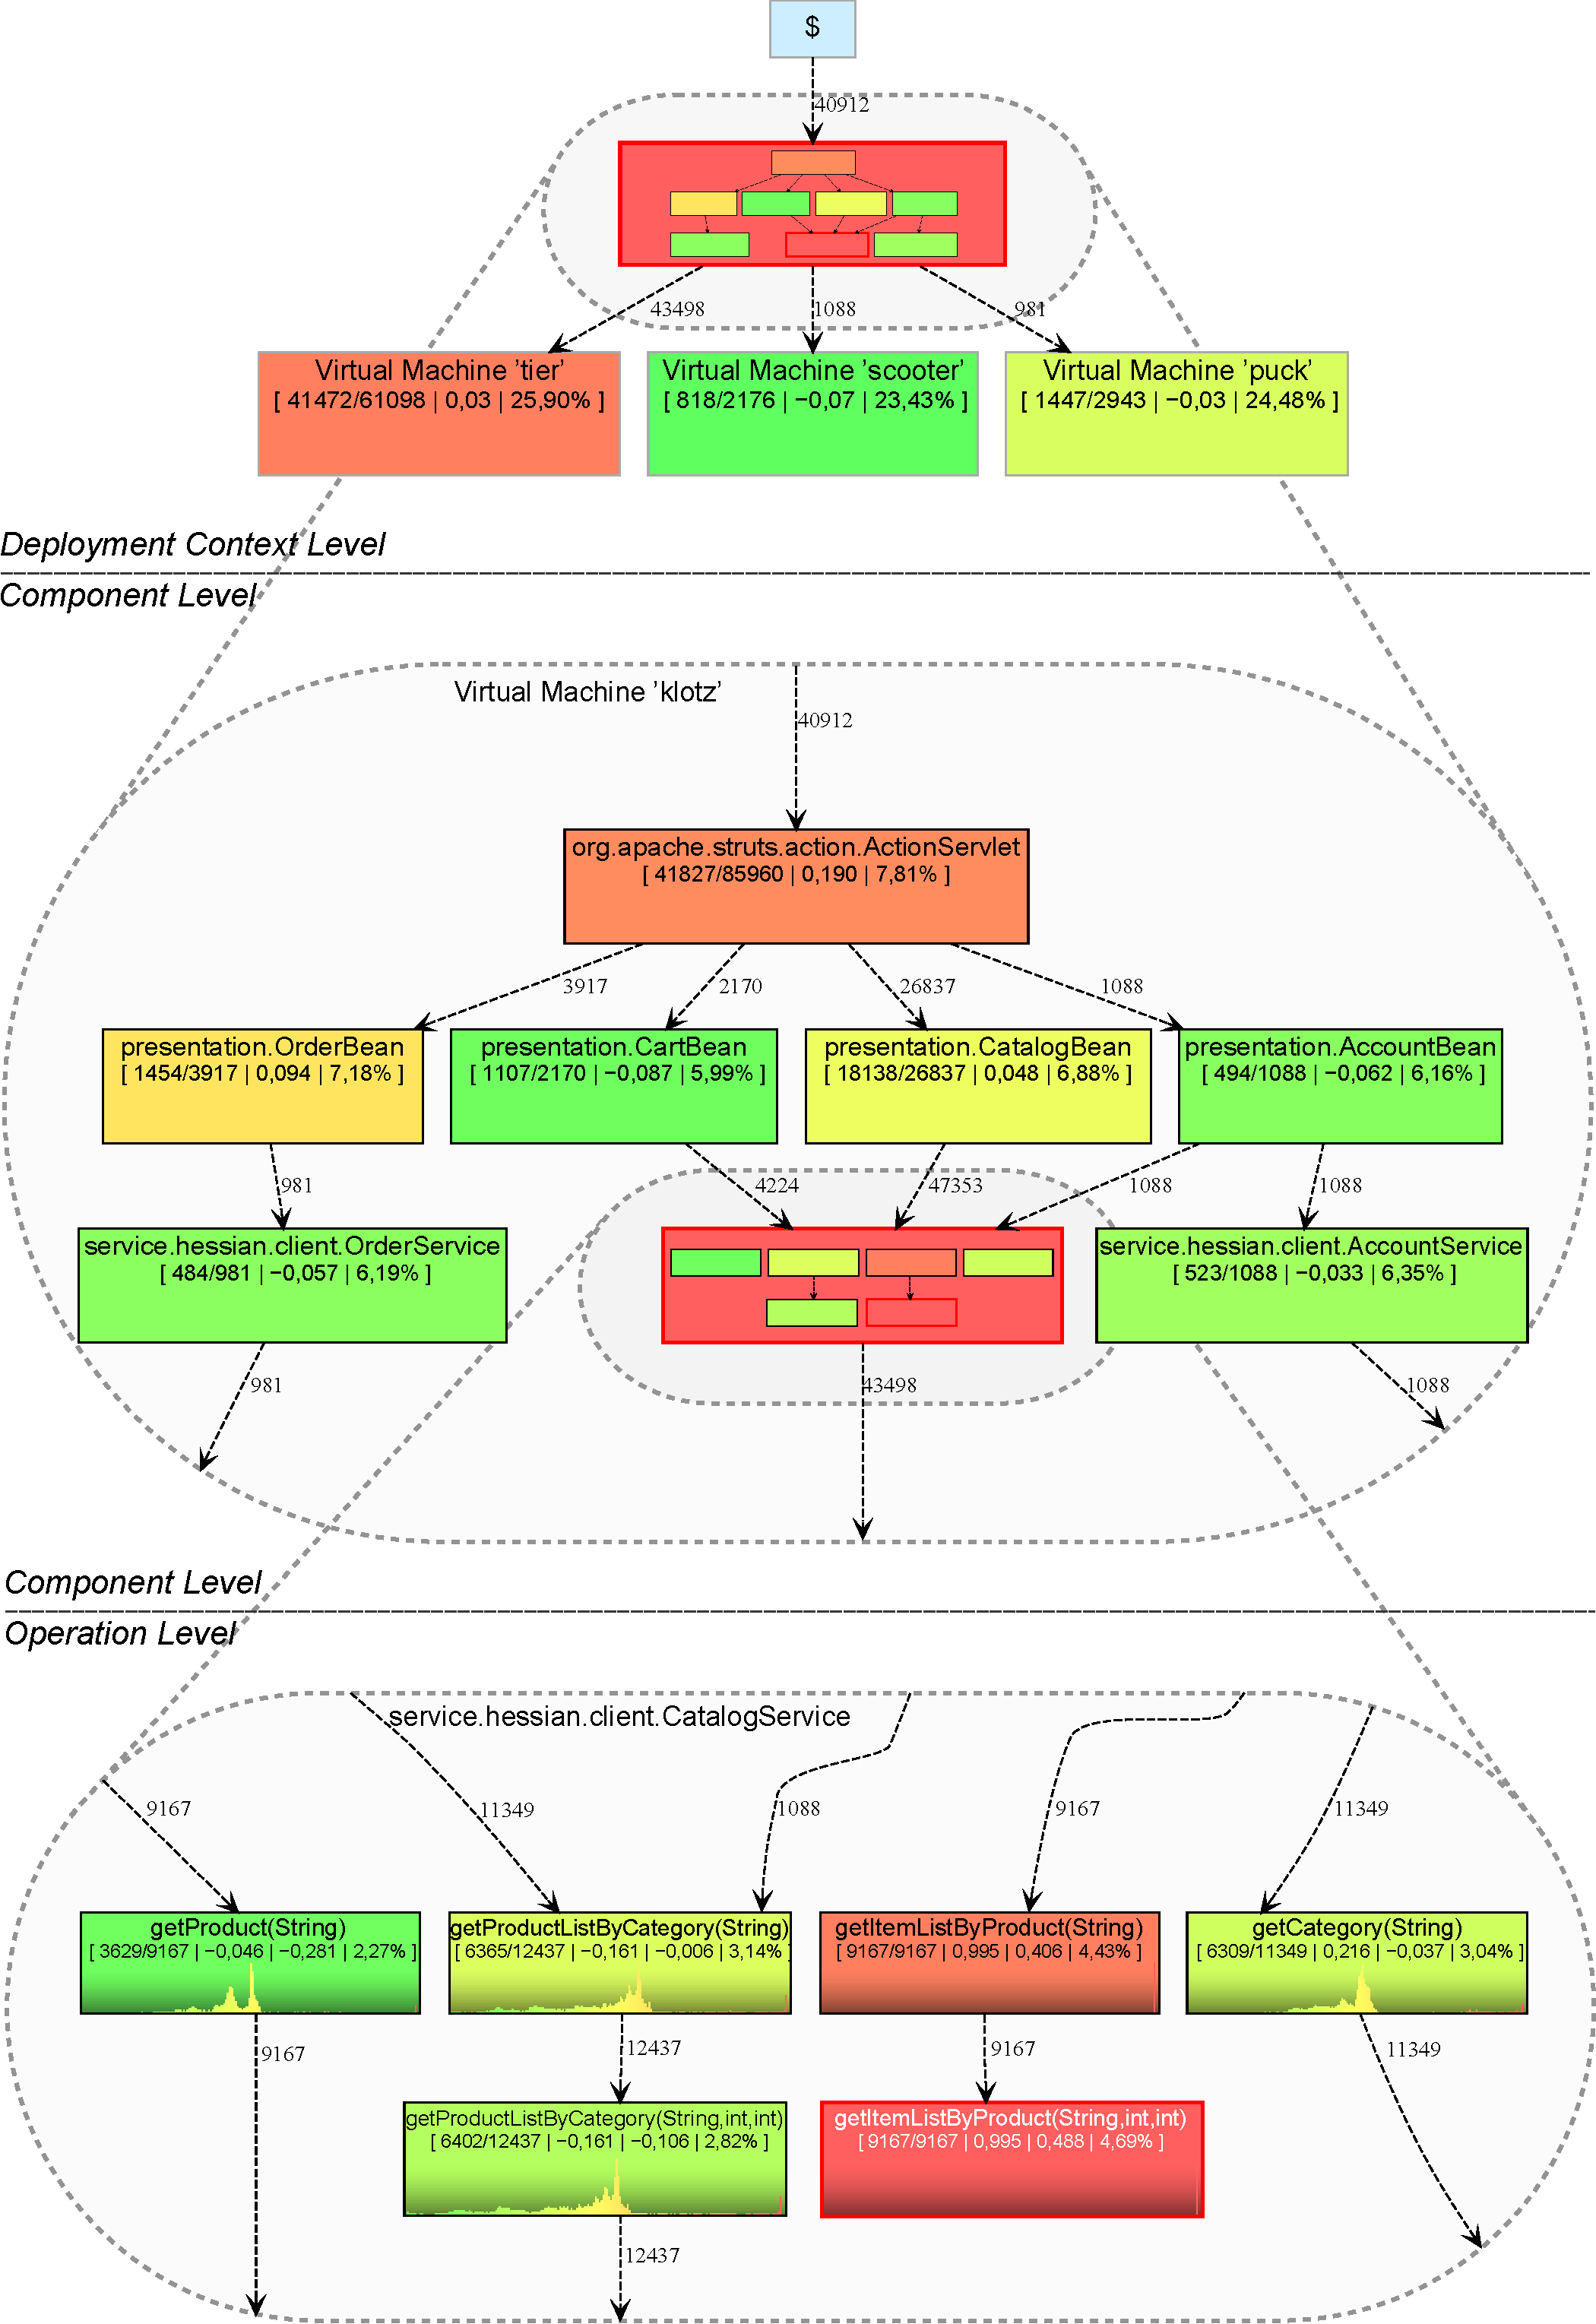
\includegraphics[width=\columnwidth]{figures/visualization-01}%
% \caption{Visualized hierarchical dependency graph~\citep{MarwedeRohrHoornHasselbring2009AutomaticFailureDiagnosisInDistributedLargeScaleSoftwareSystemsBasedOnTimingBehaviorAnomalyCorrelation}}
% \label{fig:hierarchicalDependecyGraph}
% \end{figure}
% 
% Dependency graphs are employed by some approaches to runtime reconfiguration~\citep{SEAA07} or failure %
% diagnosis~\citep{MarwedeRohrHoornHasselbring2009AutomaticFailureDiagnosisInDistributedLargeScaleSoftwareSystemsBasedOnTimingBehaviorAnomalyCorrelation}.
% Figure~\ref{fig:hierarchicalDependecyGraph} shows a dependency graph that has been enhanced with anomaly score information to support failure diagnosis. %
% In this visualization, three architectural levels (operation, component, and deployment context) are displayed and small histograms
% show the distribution of the anomaly scores for each operation. Please refer to~%
% \citep{MarwedeRohrHoornHasselbring2009AutomaticFailureDiagnosisInDistributedLargeScaleSoftwareSystemsBasedOnTimingBehaviorAnomalyCorrelation} for a detailed discussion; in the present paper this figure just serves as an illustration of possible visualizations.

% Software systems can be considered as a composition of communicating components. %
% Each component can provide some services while requiring external services. %
% A component A is dependent on component B, iff A uses/requires services provided %
% by B.  
% For illustration, %
% we extend UML component diagrams by including labeled dependencies~(see examples %
% in Figure~\ref{dependencyGraphsFigures}). The weight of an edge denotes the number %
% of actual requests for any service provided by the called component.
% 
% During runtime a system executes different scenarios and thus activates particular %
% instances of components. The runtime dependency graph among instances of components %
% at a particular point in time contains a subset of all possible dependencies of a %
% system. Considering the possibility of having a multi-user system, we can observe %
% a strong varying usage and thus varying dependencies among instances of components. %
% It is feasible to also determine the static dependency graph for the system as a %
% sum\TODO{/union?} graph from all possible execution scenarios. %Because of the problem of state explosion, we consider an experiment specific static dependency graph as a worst case runtime dependency graph for the monitored data.


% \TODOBOX{Andr\'e: Ab hier habe ich den Rest dieses Abschnitts noch
% cht \"uberarbeitet.}

% A widely used dynamic architectural viewpoint is given by UML sequence diagrams, %
% which allow to describe the interactions within object-oriented software systems. %
% A sequence diagram displays structural entities~(e.g., objects), their executions %
% (\textit{ExecutionSpecifications} in the UML) on the lifelines below them, as well %
% as call actions and returns between execution blocks.

% For this example, we partly instrumented a sample Web-based Java shopping system. %

% \begin{figure}\centering
% \includegraphics[width=0.48\textwidth]{figures/AddItemToCart2}%
% \caption{Sequence diagram}
% \label{fig:vis:seqDiagr}
% \end{figure}

% \begin{figure}\centering
% \includegraphics[width=0.48\textwidth]{figures/behaviorModel_buyer2-corrcted}%
% \caption{Markov chain}
% \label{fig:vis:markovChain}
% \end{figure}

% \begin{figure}\centering
% \includegraphics[width=0.48\textwidth]{figures/depDukeBankMockupGraph}%
% \caption{Component dependency graph}
% \label{fig:vis:dependencyGraph}
% \end{figure}

% \subsubsection{Markov chains}
% 
% \begin{figure}
%  \centering
% %trace id 3962531344010343978 database Andre table 070903_formula_fs_data
% %trace id 4148129190884353516 database Andre table 070903_formula_fs_data
% %the ``ItemSqlMapDao'' and other components with no connection were removed manually
% \includegraphics[width=0.9\columnwidth]{figures/MarkovChainBothTraces}
% \caption{Operation-level Markov chain for two message~traces~\citep{RohrHoornMatevskaStoeverSommerGieseckeHasselbring2008KiekerContinuousMonitoringAndOnDemandVisualizationOfJavaSoftwareBehavior}}
% \label{fig:vis:jpetDepMarkovChain} 
% %of the software system, generated from two Message traces that correspond to the two Sequence Diagrams
% %The states of the Markov chain represent the last message received within a particular trace and the edges point to messages that may be next with an expected probability larger than 0. The probabilities are learned from training data.
% \end{figure}
% 
% Markov chains are a common formalism used in reliability and performance theory~%
% (see e.g.~\citep{Trivedi2001ProbabilityAndStatisticsWithReliabilityQueueingAndComputerScienceApplications,MenasceAlmeidaDowdy2004PerformanceByDesignComputerCapacityPlanningByExample}) %
% to describe and analyze random processes, such as %computer 
% system and user behavior. %
% A discrete-time Markov chain describes a process in terms of a discrete number %
% of states and probabilistic transitions--in discrete time steps--among these. %
% The characteristic property of a Markov chain is that the next state of a process %
% solely depends on the process's current state. %
% An often used representation of Markov chains are (finite) state machines. %
% 
% % Markov chains provide a common stochastic means to describe dynamic system behavior %
% % of multiple scenarios. For example, Markov chains can, for instance, be used for intrusion detection %
% % to describe interactions among system components, and in reliability or performance %
% % analysis to characterize the utilization of components during service processing~\citep{GulSommerRohrVanHoornHasselbring2008EvaluationOfControlFlowTracesInSoftwareApplicationsForIntrusionDetection}. %
% % A (first order) Markov chain is a probabilistic %finite 
% % state machine with a dedicated entry and a dedicated exit state. Each transition %
% % is weighted with a probability. The sum of probabilities of outgoing transitions %
% % of a state must be $1$. Given the current state, the next state is randomly %
% % selected solely based on the probabilities associated with the outgoing transitions.
% 
% % \newpage
% 
% As illustrated in Figure~\ref{fig:vis:jpetDepMarkovChain}, Kieker can generate 
% finite state machine representations of Markov chains derived from a set of \executionTraces{}, %
% where the states represent the creation of a message within a \messageTrace{} and the edges %
% connect subsequent messages. The edges are labeled with the relative frequencies, %
% derived from the monitoring data, that messages follow each other. %
% A missing edge between two %
% messages expresses that the monitoring data analyzed contains no \trace{} with a %
% sub-sequence containing only these two messages. %
% Figure~\ref{fig:completeJpetstoreOperationProbabilityGraphAndMarkovChain} in Appendix~\ref{sec:appendix} shows %
% a single Markov chain generated from the 236\,719 traces of the JPetStore example. %
% 
% Our method used to compute Markov chains from \executionTraces{} is described %
% in~\citep{GulSommerRohrVanHoornHasselbring2008EvaluationOfControlFlowTracesInSoftwareApplicationsForIntrusionDetection}. %
% In that work, we present an application-level intrusion detection system by %
% comparing \executionTraces{} with normal behavior learned from monitoring data %
% and modeled as Markov chains. %

% %\clearpage
